%\documentclass{article}
\documentclass[prl, longbibliography]{revtex4-2}
\usepackage{graphicx}
\usepackage{makecell}
\usepackage{amsmath}
\usepackage{fontspec}
\usepackage{bbold}
%\usepackage{mathtools}
%\usepackage{mathrsfs}
\begin{document}

\title{Mark's Notes on Molecular Potential Calculations, test!}
\author{Mark O. Brown}
\date{\today}

\begin{abstract}
These notes describe the calculation of very long range S+P molecular potentials, including the leading order Bohr-Oppenheimer (BO) potentials ($1/r^3$ dipole interactions for Homonuclear S+P), fine structure, and
hyperfine structre. 
The BO potentials are diagonal in the standard Hund's "case A" molecular basis, and the fine and hyperfine structure are diagonal in the separate atom "F" angular momentum basis. 
The procedure consists of constructing the hamiltonians for each of these energies in a properly single symmetrized  basis and diagonalizing the result as a function of internuclear distance.
While it is trivial to state the procedure, identifying and keeping track of the symmetries in these calculations is rather nuanced and not clearly discussed in the literature. 
These notes therefore aim to discuss this procedure in a very pedagocial manner so that it is easy to repeat these or similar calculations without prior experience in such calculations. 
\end{abstract}

\maketitle

\section{Symmetries and quantum numbers}

\subsection{Introduction}
The symmetries of the problem are very important on a number of levels. 
In the first place, the full hamiltonian for Rb87 would be 384x384 in size, but represented in the right basis it is block-diagonal in much smaller chunks, and is therefore numerically much easier to manage. 
In addition, identifying the symmetries of the states helps to build intuition and identify patterns in the resulting molecular potentials, which have a tendency to look like spaghetti otherwise. 
Lastly, the symmetries of the state are important for identifying selection rules for the excitation of these states.

In the end, we will consider 15 different angular momentum operators and their projections on either an arbitrary axis (the "space-fixed" axis) or the molecular axis (the "body-fixed" axis). 
Not only that, but many of the labels of these angular momentum follow arcane rules established in early spectroscopy experiments.
It's therefore important that the notation here is clear and each angular momentum and projection is clearly identified. 
I will always refer to operator symbols with a hat while symbols without a hat are eigenvalues. 
Unless specifically mentioned otherwise, the eigenvalues will have the exact same symbol except without the hat. For example, $\hat{\mathbb{i}}_{e}$ is an inversion operator to be discussed later, and $i_e=\pm 1$ are the eigenvalues of this operator. 

\subsection{Separate-Atom Quantum Numbers and Interactions}
Since we will eventually be discussing two atoms, I will go ahead and add a subscript $\alpha$ which takes values either $1$ or $2$ to indicate which atom the opeartor applies to.
A single atom is spherically symmetric, and the uncoupled quantum numbers that describe it are: the principle quantum number $n_\alpha$, the orbital angular momentum $L_\alpha$, the electron spin angular momentum $S_\alpha$, and the nuclear spin angular momentum $I_\alpha$, and associated projections $m_{L_\alpha}, m_{S_\alpha}, $ and $m_{I_\alpha}$. 
This completely uncoupled basis can therefore be represented in a long ket as $|n_\alpha L_\alpha m_{L_\alpha} S_\alpha m_{S_\alpha} I_\alpha m_{I_\alpha}\rangle$.
The fine structure interaction is $\propto L_\alpha\cdot S_\alpha$ which commutes with $L^2_\alpha$ and $S^2_\alpha$ but not $L_{z\alpha}$ or $S_{z\alpha}$.
As a result, we introduce the new total single-electron angular momentum $J_\alpha=L_\alpha+S_\alpha$, and therefore we introduce the FS-coupled basis $|n_\alpha L_\alpha S_\alpha J_\alpha m_{J\alpha} I_\alpha m_{I_\alpha}\rangle$.
The Hyperfine interaction is roughly $\sim J\cdot I$, encouraging the introduction of a new total single-atom angular momentum $F_\alpha$, and we therefore introduce the HFS-coupled basis $|n_\alpha L_\alpha S_\alpha J_\alpha I_\alpha F_\alpha m_{F_\alpha}\rangle$. 
This is the basis typically used for atomic physics, although depending on the context it is common to omit many of these extraneous uncoupled quantum numbers. 
For example the common label for fine structure manifolds is $^{2S+1}L_J$, where $L$ is replaced by S for $L=0$, P for $L=1$, D for $L=2$, etc.

\subsection{Bohr-Oppenheimer Symmetries}
Introducing a second atom breaks the spherical symmetry of a single atom.
Many of the remaining symmetries are spatial symmetries of the problem respecting various aspects of the cylindrical symmetry of the problem, so for discussions of the coordinates of the particles in the problem we will consider our coordinate system to be such that the center of mass and charge is at the origin, and the intermolecular axis is aligned along the z-axis. 
Thankfully, for homonuclear atoms the center of charge is the same as the center of mass of the molecule, and so we avoid some minor complications which are encountered with heteronuclear molecules.
Therefore, we start here with the symmetries that are valid with BO interactions but without FS or HFS interactions, and will then work to build the FS and HFS interactions back into the problem.

In general, the interactions between the atoms couples states of different $n_\alpha$ and $L_\alpha$, so none of these are good quantum numbers anymore. In addition, the orientation of the molecule is the only axis of symmetry in the problem, and so only the projection of the angular momentum in the problem which is conserved is that along the internuclear axis. 
In general, since $L_\alpha$ aren't good quantum numbers, it only makes sense to consider the total projection of both angular momentum along this axis, which is typically defined as $\Lambda=L_{1z}+L_{2z}$. 
In general, I will follow the pattern that projections along arbitrary axes, for example in the separate atom case above, are represented by $m$ subscripted with the lattin letter corresponding to its angular momentum (e.g. $m_L$), whereas projections that are specifically along the molecular axis will always be represented by greek letters.
Furthermore, similar to the way L is replaced by S, P, D, etc. for single atom labels, $\Lambda$ will be represented as $\Sigma$ if $\Lambda=0$, $\Pi$ if $\Lambda=1$, $\Delta$ if $\Lambda=2$, etc.

The BO interactions are primarily based on the electric interactions of the electrons with each other and the two nuclei, so BO states still have good values of the total electron spin $S=S_1+S_2$, and can be therefore classified by this quantum number.



\subsection{Geometric Symmetries}

Homonuclear molecules belong to the point group $D_{\infty h}$, which provides for an easy baseline to discuss the relevant symmetries here for the mathematically inclined. 

The problem is symmetric under the \emph{inversion} of all of the electronic spatial coordinates. 
I define the inversion operator which does this as $\hat{\mathbb{i}}_e$.
Since swapping these coordinates twice brings us back to the original state, states can either be symmetric or antisymmetric under this inversion. 
Symmetric states are typically referred to as \emph{gerade} (or "g") or \emph{ungerade} ("u") states. 

Finally, the problem is also symmetric under the reflection of the electrons spatial wavefunction across a plane \emph{containing} the internuclear axis, for example the xz plane, which would be equivalent to setting $y_1\rightarrow -y_1$ and $y_2\rightarrow-y_2$ or $\phi\rightarrow -\phi$ where $\phi$ is the polar angle in spherical coordinates.
The operator which does this is typically labeled $\sigma_v$, however since we will have to modify the operator several times as we add fine and hyperfine structure, I represent this operator which only changes the spatial coordinates of the electron as $\hat{\sigma}_{v_L}$ since it doesn't touch the spin. For any state with Quantum numbers $L$ and $\Lambda$, the operation of $\sigma_{v_L}$ is:

$$
\sigma_{v_L}|L\Lambda\rangle = (-1)^{L-\Lambda}|L,-\Lambda\rangle
$$

Similar to the inversion operator, we must have $\sigma _{v_L}=\pm 1$. This symmetry is slightly counterintuitive from an atomic perspective since the normal hydrogen atom wavefunctions are not eigenvalues of this operator. 
This is simply the result of the choice of basis for the functions however, and one can construct good such states easily enough. For example, with an abbreviated uncoupled basis $|n_\alpha L_\alpha m_{L_\alpha}\rangle$, the superpositions $|111\rangle \pm |11,-1\rangle$ are eigenstates of this reflection operator.
Such symmetric states are typically labeled with a $+$ and antisymmetric states with a $-$. While all BO states can be constructed as eigenstates of this operator, if $\Lambda\ne 0$ the states with different reflection parity are degenerate, and this label is sometimes dropped in those circumstances.

There are a number of additional symmetries one can identify for these potentials involving the other uncoupled angular momentum. For example, states that have different projections of the total spin along the internuclear axis (defined as $\Sigma=S_{1z}+S_{2z}$). However, the symmetries already defined are more than enough to identify all the non-degenerate potentials at this level.

Therefore, BO states are typically labeled by four characters representing the values of $2S+1$, $\Lambda$, $\mathbb{i}_{e}$, and $\sigma_{v_L}$ oriented like this $^{2S+1}\Lambda^{\sigma_{v_L}}_{\mathbb{i}_e}$. For example, with $S=1,\Lambda=0,\mathbb{i}_e=1,\sigma_{v_L}=1$, the symbol is $^3\Sigma_g^+$. In addition, even including all values of $\Lambda$ is unnecessary, as states with positive and negative values are degerate, and so typically only the absolute value of Lambda is reported despite it being possible to have negative values of this quantum number.

It is worth noting now, in the far-separated regime we are interested in, the mixing of states with different $L_\alpha$ and $n_\alpha$ is very weak, and the leading order interactions can be modeled as the dipole-dipole interactions between states that do have well defined $L_\alpha$ and $n_\alpha$. So, in the calculations that follow, the bases that are used will have well-defined $L_\alpha$ and $n_\alpha$. 

\subsection{BO with Fine Structure}

Adding the fine structure, similar to the separate atom case, means that $\Lambda$ and $\Sigma$ are no longer good quantum numbers, but that $\Omega=J_{1z}+J_{2z}$ is a good quantum number now. However, similar to the previous case, only the absolute value of $\Omega$ matters. Unlike for $\Lambda$, in the symbols for these states $\Omega$ are just the numeric value of $|\Omega|$. 

In addition, because the fine structure couples states of different $L$ and $S$, the fine-structure interaction inadvertedly also couples states of different values of $\sigma_{v_L}$, making it also not a good quantum number. However, the operator which flips both the spatial component of the the electronic wavefunction \emph{as well as the spin} (effectively flipping both $\hat{L}$ and $\hat{S}$) commutes with the fine structure hamiltonian and will give us good quantum numbers. I will label this slightly different operator $\sigma_{v_{LS}}$. Similarly to the previous case, it is only states with $\Omega=0$ that states with different $\sigma_{v_{LS}}$ are not degenerate.

$$
\sigma_{v_{LS}}|L\Lambda S \Sigma\rangle = (-1)^{L-\Lambda+S-\Sigma}|L,-\Lambda S, -\Sigma\rangle
$$

$i_e$ are still good quantum numbers. Therefore, the symbols for these types of states are of the form $\Omega_{i_e}^{\sigma_{v_{LS}}}$, for example $0_g^+$.

\subsection{BO with Hyperfine Structure}

Adding the hyperfine structure follows a similar pattern as with adding the fine structure. In this case, our good projection is now the projection of the total atomic angular momentum defined as $\phi=F_{1z}+F_{2z}$. Similarly, only the absolute value of $\phi$ matters. 

The hyperfine interaction hamiltonian couples states of different $\sigma_{v_{LS}}$, and so we must modify this reflection operator again to have good quantum numbers. Now, if an operator also flips the nuclear spin in addition to the electronic spin and spatial wavefunction, this will commute with our total hamiltonian. Since this is our final reflection operaotr, I will give this one the nice symbol $\sigma_v$. 

$$
\sigma_{v_L}|L\Lambda S \Sigma I \iota\rangle = (-1)^{L-\Lambda+S-\Sigma+I-\iota}|L,-\Lambda, S, -\Sigma, I, -\iota\rangle
$$

Because we are now considering the nuclear spin, the two nuclear centers are now not necessarily identical, and so now $i_e$ are no longer good quantum numbers. We can construct a similar operator however which inverts both the electrons spatial coordinates as well as the nuclear spatial coordiantes. I will represent this final inversion operator with the nice symbol $\hat{i}$. 

Notation for the labels of these states with molecular potentials is not particularly well established. In the past, Jose and his collaborators have labeled states with $i=1$ as "a" states and states with $i=-1$ as "b" states. As well, they referred to states with $\sigma_v=1$ as "1" states and $\sigma_v=2$ as "2" states. As such, their labels were of the form $\phi i \sigma_v$. I will avoid this convention for these notes (at least for now, perhaps someone will convince me otherwise :)). Since there is such a wealth of confusing notation here, I will opt for a very explicit notation in these notes. States with $i=\pm 1$ will be labeled "$i\pm$", and states with $\sigma_v=\pm1$ will be labeled $\sigma\pm$, in the convenient notation $\phi_i^{\sigma_v}$. The states relevant for Rb87 calculations are then $0_{i+}^{\sigma_v+},0_{i+}^{\sigma_v-},0_{i-}^{\sigma_v-},0_{i+}^{\sigma_v-}, 1_{i+},1_{i-},2_{i+},2_{i-},3_{i+},3_{i-},4_{i+},4_{i-},5_{i+},5_{i-}$. One fairly sensible alternative here is to drop the $i$ and $\sigma_v$ from the labels, and instead label them like $0^+_-$

\begin{center}
\begin{tabular}{ ||c|c|c|c|c|c||  }
 \hline
 Description & \makecell{Angular \\Momentum \\Operator $\hat{Z}$} & \makecell{$\hat{Z}^2$ Eigenvalues \\($\hbar^2 z(z+1)$)} & \makecell{Body-Fixed\\ $\hat{Z}_z$ Eigenvalues \\($\hbar m_z$)} &\makecell{Space-Fixed\\ $\hat{Z}_z$ Eigenvalues \\($\hbar m_z$)} & \makecell{Alternative\\Operator\\Representations}\\
 \hline
 \hline
 Single Electron Orbital A.M. & $\hat{L}_\alpha$ & $L_\alpha$ & $\Lambda_\alpha$ & $m_{L_\alpha} $ & None \\
 \hline
 Total Electron Orbital A.M. & $\hat{L}$ & $l$ & $\Lambda=\Lambda_1+\Lambda_2$ &$m_L $ & $\hat{L}=\hat{L}_1 + \hat{L}_2$ \\
 \hline
 Single Electron Spin & $\hat{S}_\alpha$ & $S_\alpha$ & $\Sigma_\alpha$ &$m_{S_\alpha} $ & None \\
 \hline
 Total Electron Spin & $\hat{S}$ & $S$ & $\Sigma=\Sigma_1+\Sigma_2$ &$m_S $ &  $\hat{S}=\hat{S}_1 + \hat{S}_2$ \\
 \hline
 Single Electron Total A.M. & $\hat{j}_\alpha$ & $j_\alpha$ & $\Omega_\alpha=\Lambda_\alpha+\Sigma_\alpha$ &$m_{j_\alpha} $ &  $j_\alpha = L_\alpha+S_\alpha$ \\
 \hline
 Total Electron A.M. & $\hat{j}$ & $j$ & $\Omega=\Lambda+\Sigma$ &$m_j $  & $\hat{j} = \hat{L}+\hat{S}$ \\
 \hline
% Total A.M. Except Nuclear Spin & $\hat{J}$ & $J$ & Also $\Omega$ &$m_J $  & $\hat{J}=\hat{L}+\hat{S}+\hat{N}$ \\
% \hline
% Nuclear Rotational A.M. & $\hat{N}$ & $\ell$ & $0$ (Always) & $\mu$ &  $\hat{N} = \hat{J} - \hat{L} - \hat{S}$ \\
% \hline
 Single Nuclear Spin & $\hat{i}_\alpha$ & $i_\alpha$ & $\iota_{\alpha}$ &$m_i $ &  None \\
 \hline
 Total Nuclear Spin & $\hat{I}$ & $I$ & $\iota=\iota_1+\iota_2$ &$m_I $ &  $\hat{I}=\hat{i}_1+\hat{i}_2$ \\
% \hline
% \makecell{Total Mechanical A.M.\\(Relevant in Hund's cases (b) and (d))} & $\hat{K}$ & $K$ & (Rare)$\kappa$? &$m_K $ &  $\hat{K}=\hat{L}+\hat{N}$ \\
 \hline
  Single Atom Total A.M. & $\hat{f}_\alpha$ & $f_\alpha$ & $\phi_\alpha=\Omega_\alpha+\iota_{\alpha}$ &  $m_{f_\alpha} $& $\hat{f}_\alpha=\hat{j}_\alpha+\hat{i}_\alpha$ \\
 \hline
   Total Non-Rotatoinal A.M. & $\hat{f}$ & $f$ & $\phi=\Omega+\iota$ &  $m_f $& $\hat{f}=\hat{j}+\hat{i}$ \\
 \hline
%  Total A.M. & $\hat{F}$ & $F$ & Also $\phi$ &$m_F $ &  $\hat{F}=\hat{J}+\hat{I}$ \\
% \hline 
\end{tabular}
\end{center}

\section{calculation}

\section{Selection Rules}
Currently most of my thoughts on selection rules are coming from "Herzberg" - Spectra of diatomic molecules. It seems most likely that the obvious extensions of selection rules hold in the case of hyperfine interactions holding without rotation. That is: $\phi'=\phi+\{0,\pm 1\}$, $\mathbb{i}\pm\leftrightarrow\mathbb{i}\mp$, and $\sigma_v\pm\leftrightarrow\sigma_v\pm$ for states that have well-defined $\sigma_v$. 

\section{Rotation}

Loading experiments are in a unique regime where rotational energy is small compared to all other energy scales. In many molecular experiments, the rotational energy is significant even compared to the fine structure energy scale. The rotational kinetic energy of a rigid rotor is given by $\hbar^2 \ell (\ell+1)/(m_{Rb^{87}}R^2)$ where $R$ is the internuclear distance. Fundamentally, since the loading occurs during sub-doppler cooling, the values this rotational kinetic energy takes are on the order of a couple MHz, and are naturally far below the linewidth of the molecular states involved, and as well much smaller than the hyperfine structure, which is tens to hundreds of MHz large in Rubidium. In general, the coriolis force will mix states of good hyperfine symmetry, but in this region this mixing is small and so states should maintain . This limits the maximum values of $\ell$ available at a given distance. More importantly, the collisions happen at relatively large distance scales, where $R$ is on the order of 10s of nm. Using this info, we can estimate the rotational energy splittings at a given distance as well. The result is displayed in the figure below. It's easy to see that at the distance and energy scales relevant for collisions, the rotational splittings are all well sub-linewidth. As such, they are not resolvable and only contribute to a small extra broadening of the states. We have determined that rotation does not mix states significantly, and rotational levels are not resolvable, therefore we can ignore rotation.

I think the part of this argument that I'm least convinced of is that the energies are necessarily low, since it's not literally the rotational energy which appears in the hamiltonian, but I think the actual elements should be on this order. 

\begin{figure}
  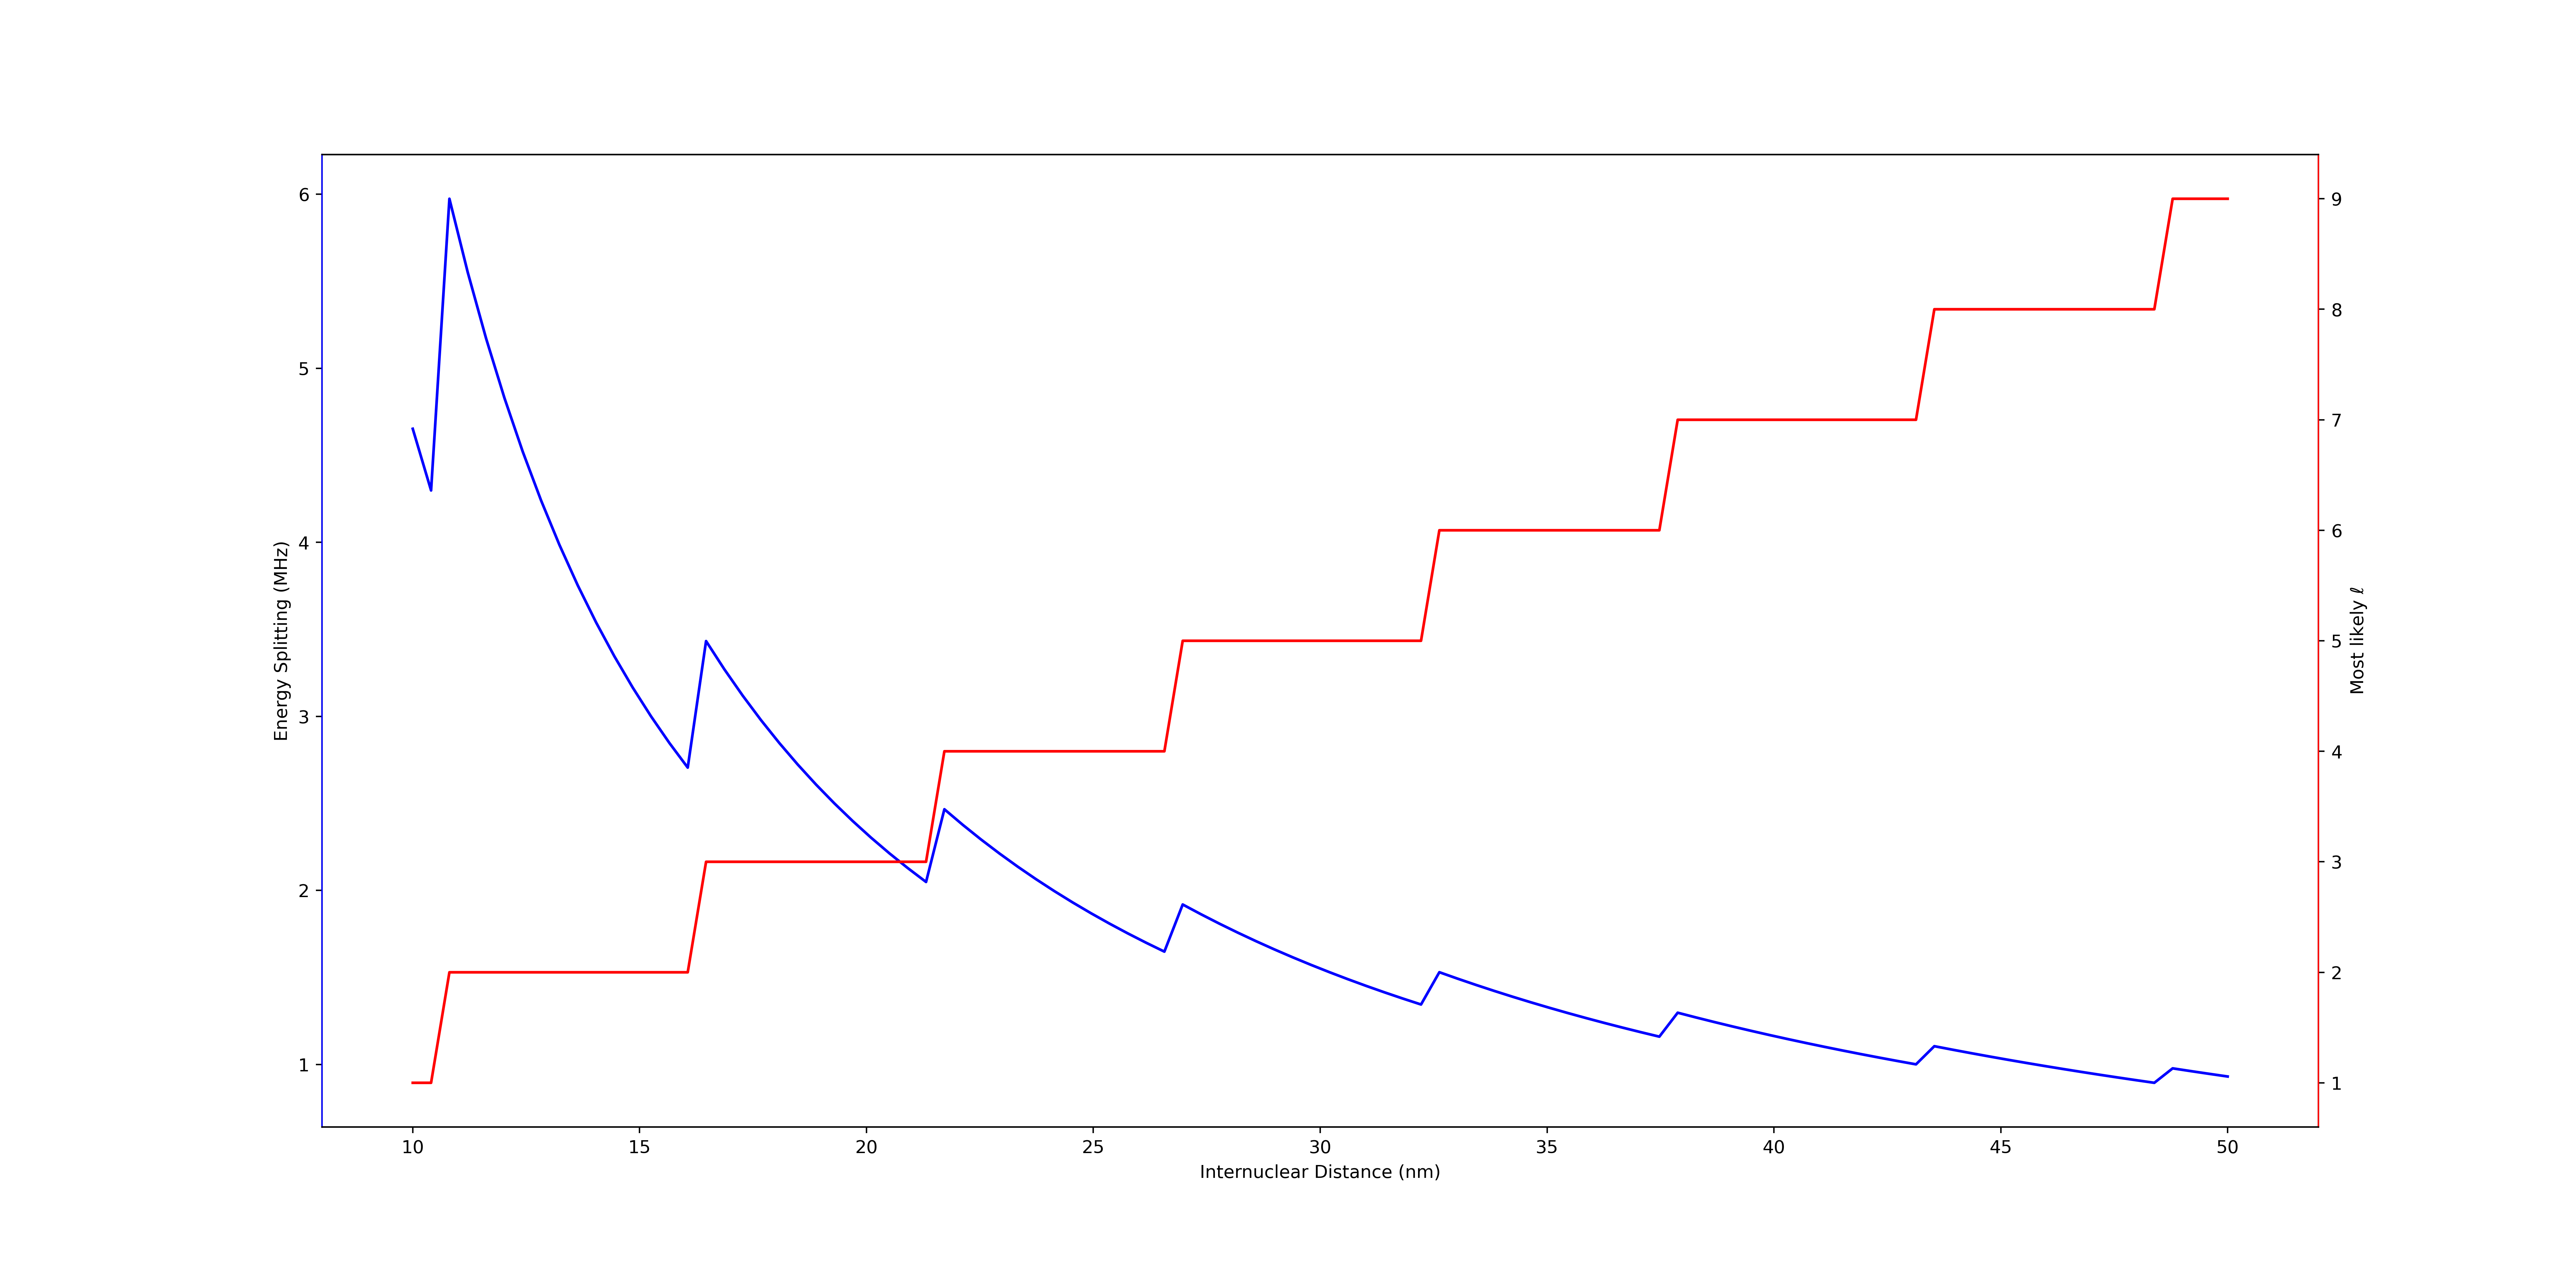
\includegraphics[width=\linewidth]{Rotational_Energy_Separation.png}
  \caption{Rotational Energy Separation Figure.}
  \label{fig:boat1}
\end{figure}

\bibliography{ShortBib}

\end{document}
